\documentclass[12pt]{report}
\usepackage{graphicx}
\usepackage[utf8]{inputenc}
\usepackage[spanish]{babel}
\usepackage{setspace}
\usepackage{geometry}
\usepackage{titlesec}
\usepackage{times}
\usepackage{mathptmx} % Use mathptmx instead of times
\usepackage{fancyhdr}
\usepackage{float}
\usepackage{pdfpages}



% Configuración de márgenes
\geometry{
    top=2.5cm,
    left=3cm,
    right=3cm,
    bottom=2.5cm
}

% Configuración de interlineado
\onehalfspacing

% Configuración de títulos y subtítulos
\titleformat{\chapter}[display]
  {\normalfont\bfseries\centering}{}{0pt}{\fontsize{14}{16}\selectfont}
\titleformat{\section}
  {\normalfont\bfseries}{\thesection}{1em}{\fontsize{12}{14}\selectfont}
\titleformat{\subsection}
  {\normalfont\bfseries}{\thesubsection}{1em}{\fontsize{12}{14}\selectfont}


% Configuración de pie de página
  \fancyhf{}
\fancyfoot[R]{\thepage}
\pagestyle{fancy}
\fancypagestyle{plain}{
  \fancyhf{}
  \fancyfoot[R]{\thepage}
}

  \begin{document}
  \pagenumbering{roman}
%----- PORTADA ----
\setlength{\hoffset}{27 pt} % 1 (Para centrar más la portada)
\begin{titlepage}
{\centering
{\fontfamily{ptm}\scshape\bfseries\fontsize{29.16}{34.992}\selectfont Universidad de Guadalajara \par}
\vspace{0.5cm}
{\scshape\Large Centro Universitario de los Lagos \par}
\vspace{1cm}
{\scshape\Large División de Estudios de la Biodiversidad e innovación Tecnológica \par}
\vspace{1cm}
{\graphicspath{{imagenes/Portada}} %ruta de las imagenes

\includegraphics[width=0.3\textwidth]{image.png}\par}
\vspace{1cm}
% Título
{\scshape\large\bfseries Practica 3: CIRCUITO INTERLOCK
DOMINANTE ON Y DOMINANTE OFF \par}
\vspace{0.5cm}
% Materia
{\large \textbf{Materia:} \\Controladores Lógicos Programables\par}
\vfill
% Estudiante
{\large \textbf{Presenta:} \\Oscar Iván Moreno Gutiérrez \#220942754
\\Maximiliano Frias Campos \#217488066
\par}
\vfill
% Profesor
{\large \textbf{Profesor:} \\Dr. Afanador Delgado Samuel Mardoqueo \par}
\vfill
\vfill
% Fecha
\begin{flushright}
  {\normalsize \textbf {Fecha:} \\ \today}
\end{flushright}
\vfill}
{\large  \par}
\end{titlepage}
%----- FIN DE PORTADA ----

%----- ÍNDICE GENERAL ----
\tableofcontents
\newpage

%----- PALABRAS CLAVE ----
\pagenumbering{arabic}
\chapter*{Palabras Clave}
\begin{itemize}
   \item Interlock: Un mecanismo de seguridad que impide la operación simultánea de ciertos componentes.
   \item PLC: Controlador Lógico Programable, un dispositivo utilizado para automatizar procesos industriales.
   \item Circuitos de control: Sistemas eléctricos diseñados para gestionar y controlar el funcionamiento de otros dispositivos.
\end{itemize}
\addcontentsline{toc}{chapter}{Palabras Clave}
%\begin{itemize}

%\end{itemize}
\newpage

%----- OBJETIVO ----
\chapter*{Objetivo}
\addcontentsline{toc}{chapter}{Objetivo}
El objetivo de esta práctica es comprender el funcionamiento y la importancia del circuito interlock en los sistemas de control, donde es crucial gestionar el encendido no simultáneo de múltiples salidas. A través de esta práctica, se busca afianzar los conocimientos teóricos y prácticos sobre la implementación y simulación de circuitos interlock, destacando su relevancia en aplicaciones industriales.
\newpage

%----- CONTENIDO ----
\chapter{Contenido}
\section{Que es un circuito de interlock?}
El interbloqueo eléctrico es un mecanismo de controles y dispositivos eléctricos diseñado para asegurar la operación segura y ordenada de circuitos eléctricos, maquinaria o equipos, evitando ciertas acciones o condiciones a menos que se cumplan requisitos específicos. Por ejemplo, cuando se necesita realizar una operación de inversión de motor controlada por dos contactores, solo uno de los contactores debe estar operativo a la vez para prevenir daños en el circuito. Nos basameros en la figura \ref{fig:interlock} para la realización de la práctica.
\begin{figure}[H]
  \centering
  \includegraphics[width=0.5\textwidth]{screenshots/circuito_interlock.png}
  \caption{Circuito de interlock}
  \label{fig:interlock}
\end{figure}

\section{Materiales}
Para la realización de esta práctica se utilizaron los siguientes materiales:

\begin{itemize}
  \item \textbf{Aplicación con picosoft:} Software utilizado para la simulación y programación de PLCs.
  \item \textbf{PLC:} Controlador Lógico Programable utilizado para la implementación del circuito.
  \item \textbf{Botonera:} Dispositivo que contiene los botones de arranque y paro.
  \item \textbf{Botones:} Componentes individuales de la botonera utilizados para controlar el circuito.
\end{itemize}

\section{Procedimiento}
\begin{enumerate}
  \item Simulamos el circuito interlock.
  \begin{enumerate}
    \item Creamos las variables de entrada y salida. (Vease la figura \ref{fig:variables})
    \begin{figure}[H]
      \centering
      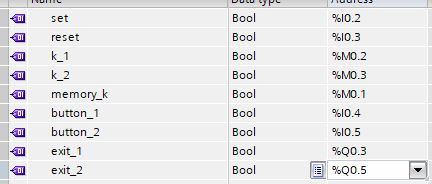
\includegraphics[width=0.5\textwidth]{screenshots/variables.png}
      \caption{Variables de entrada y salida}
      \label{fig:variables}
    \end{figure}
    \item Cremos el circuito de interlock.
    \begin{center}
      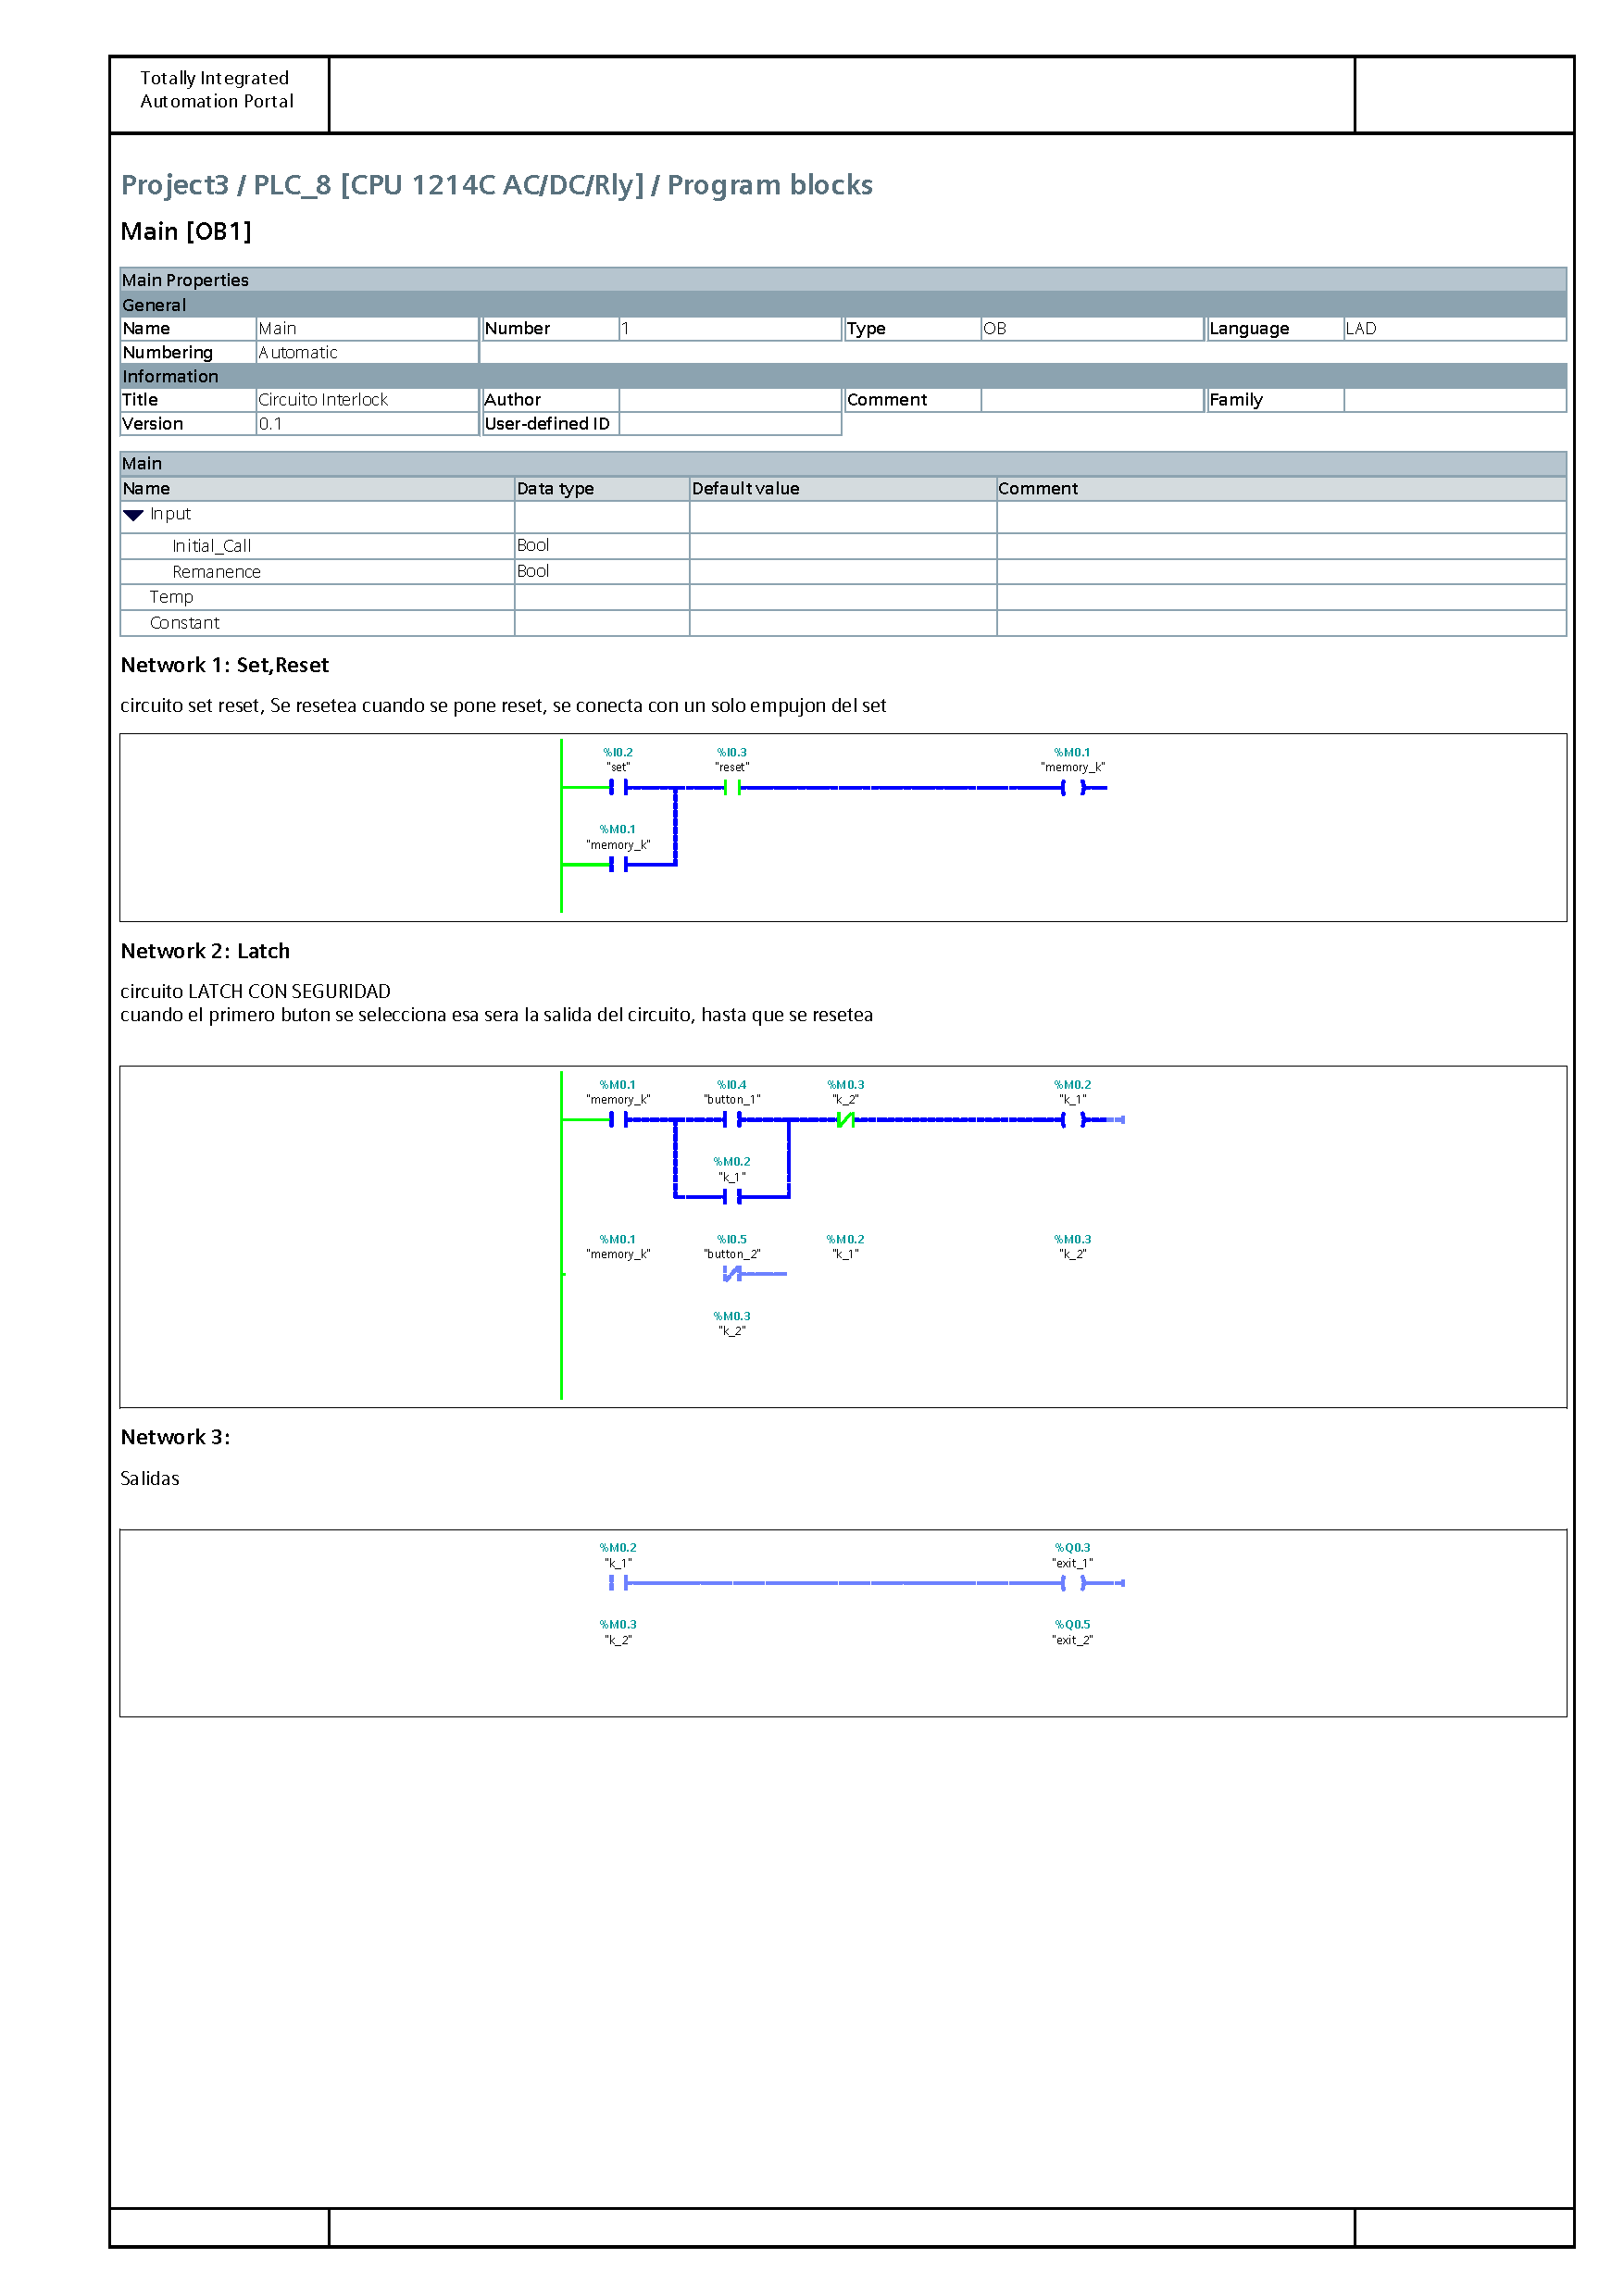
\includepdf[scale=0.9]{screenshots/practica3.pdf}
    \end{center}
  \end{enumerate}
  \item Probamos el efecto de bloqueo mutuo (interlock). Activamos una de las salidas y luego seguido intentamos activar la otra salida.
  \begin{figure}[H]
    \centering
    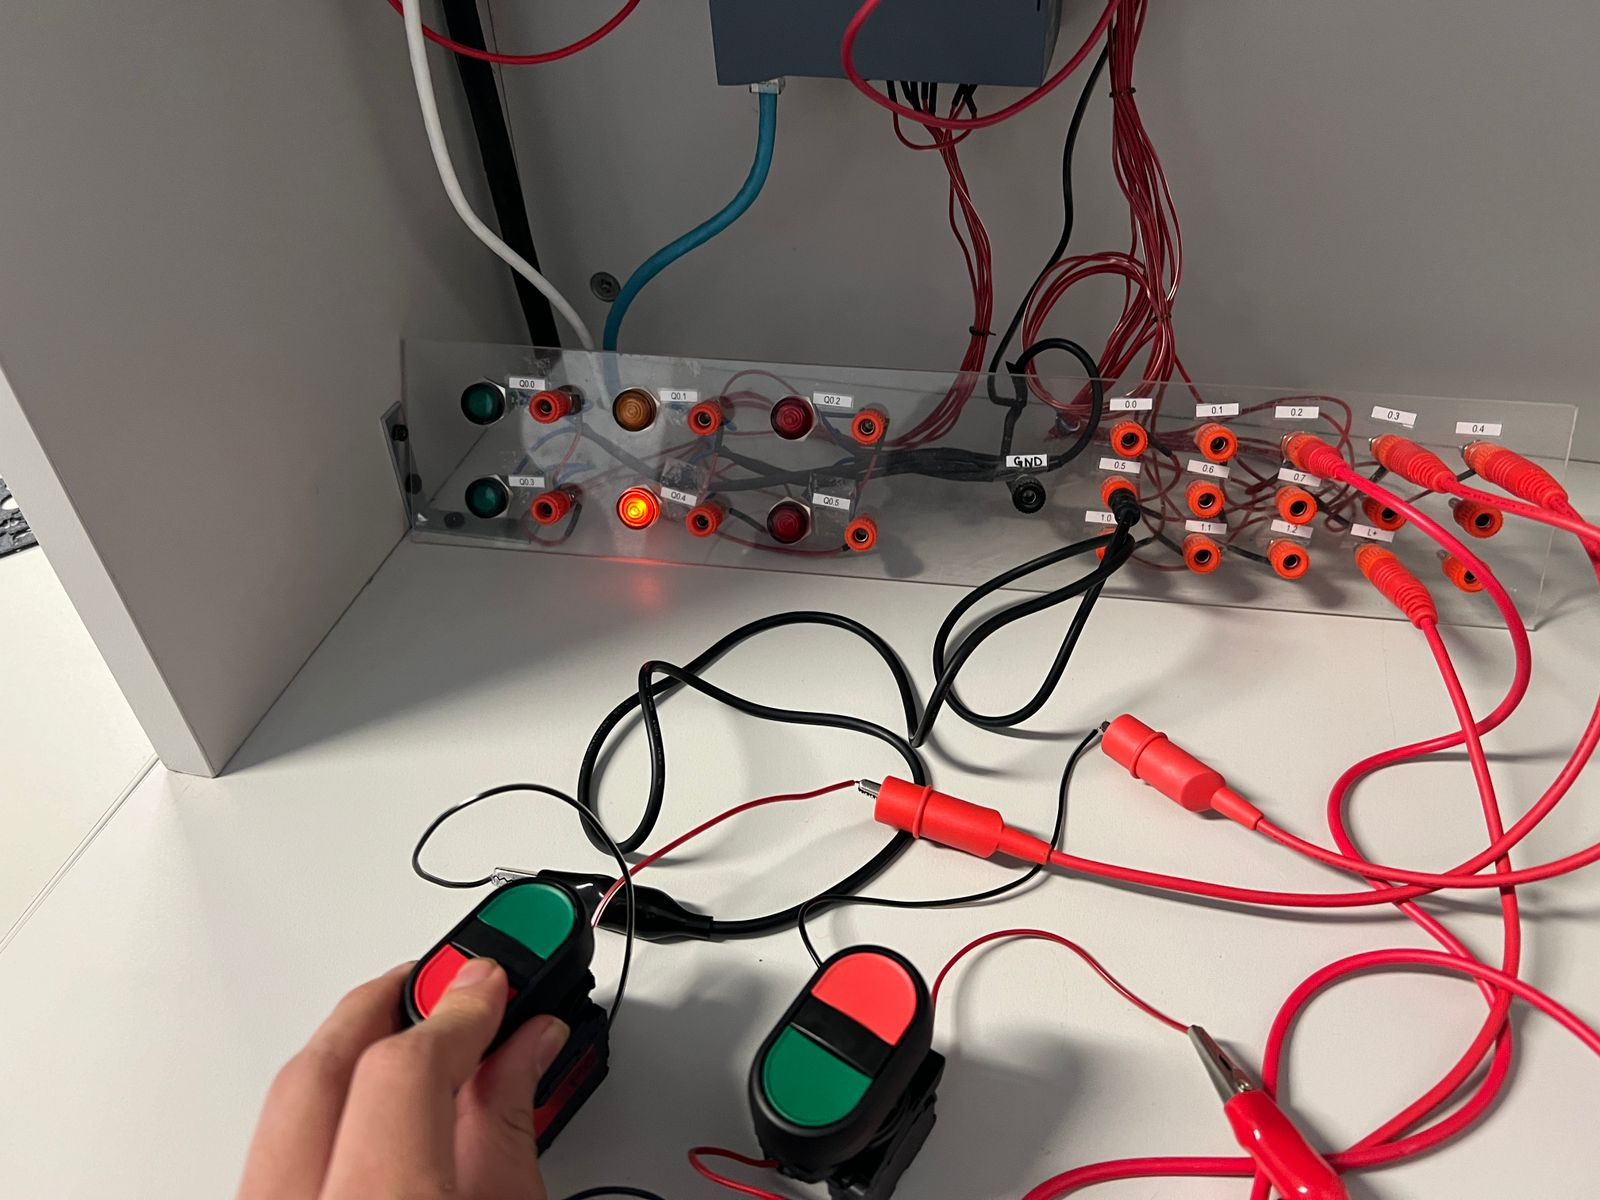
\includegraphics[width=0.5\textwidth]{screenshots/imagen_1.jpg}
    \caption{Salida 1 activada}
    \label{fig:salidas_1}
  \end{figure}
  \item Detenemos el circuito con el boton de paro y probamos encendido la otra salida primero y procedemos a intentar encender la salida contraria.
  \begin{figure}[H]
    \centering
    \begin{minipage}[b]{0.45\textwidth}
      \centering
      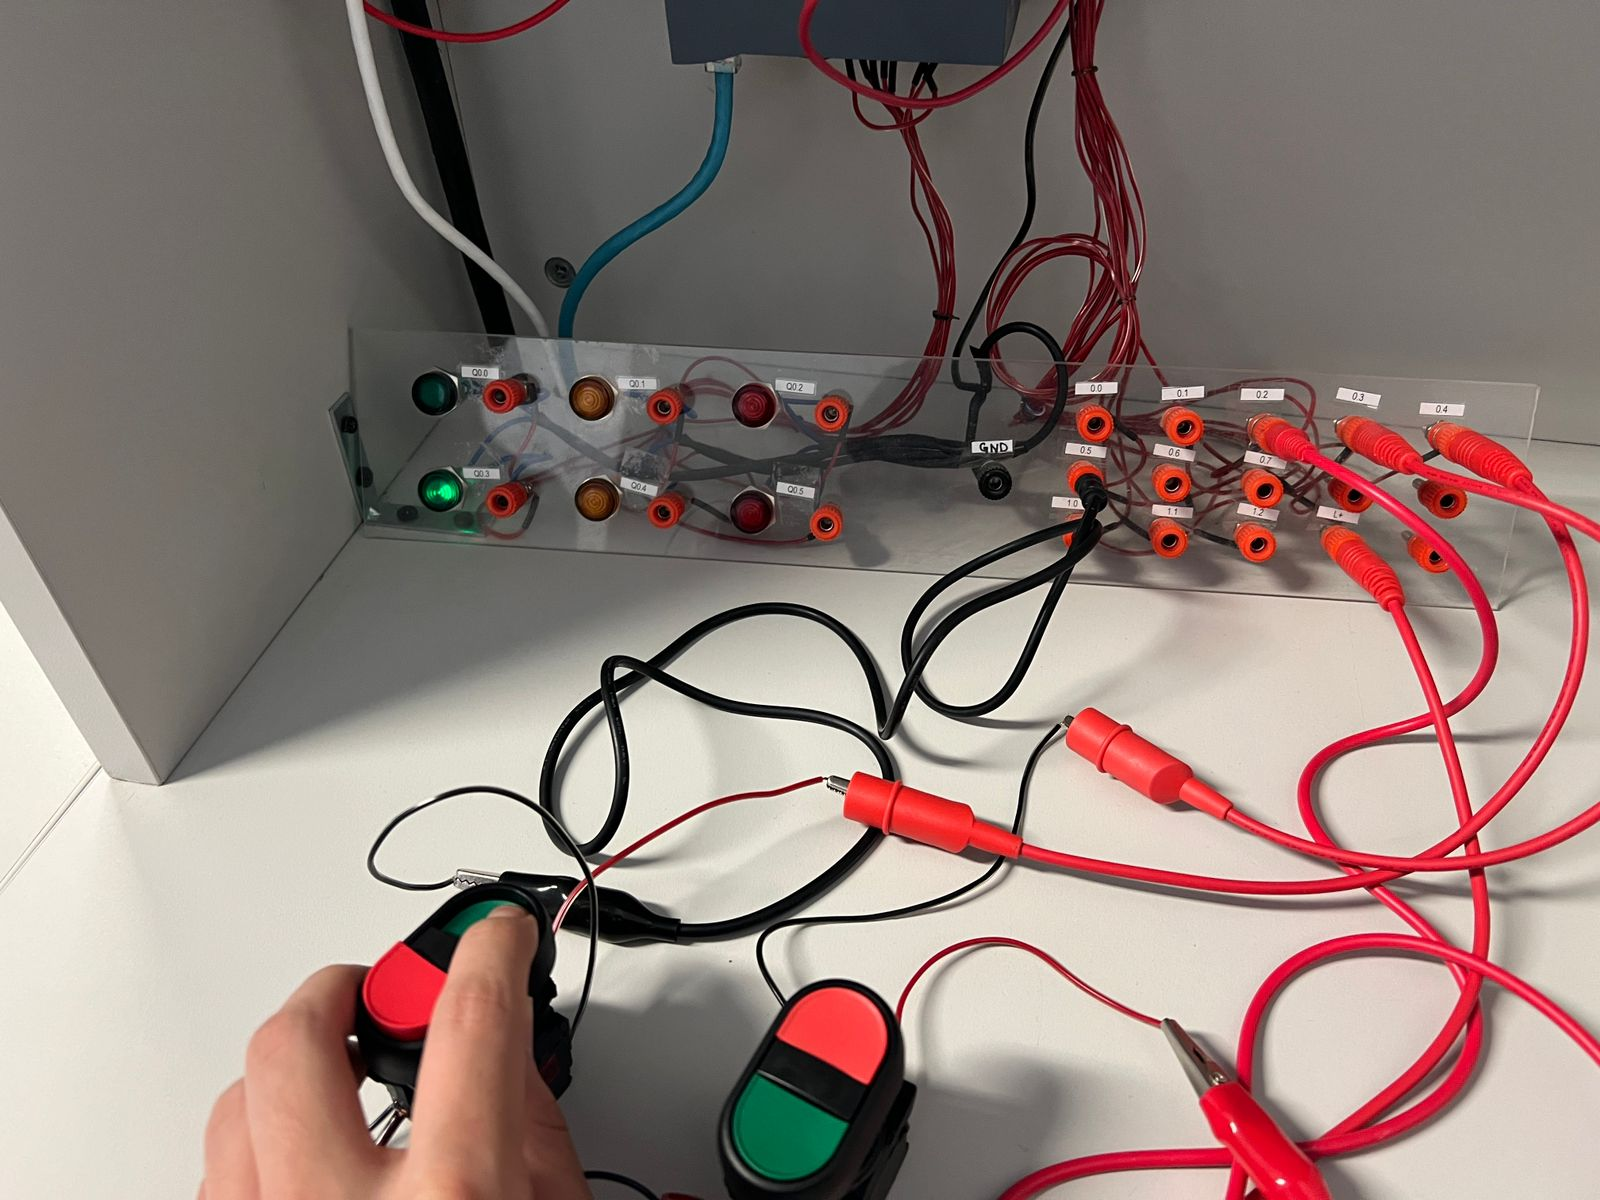
\includegraphics[width=\textwidth]{screenshots/imagen_3.jpg}
      \caption{Salida 1 activada}
      \label{fig:salidas_2}
    \end{minipage}
    \hfill
    \begin{minipage}[b]{0.45\textwidth}
      \centering
      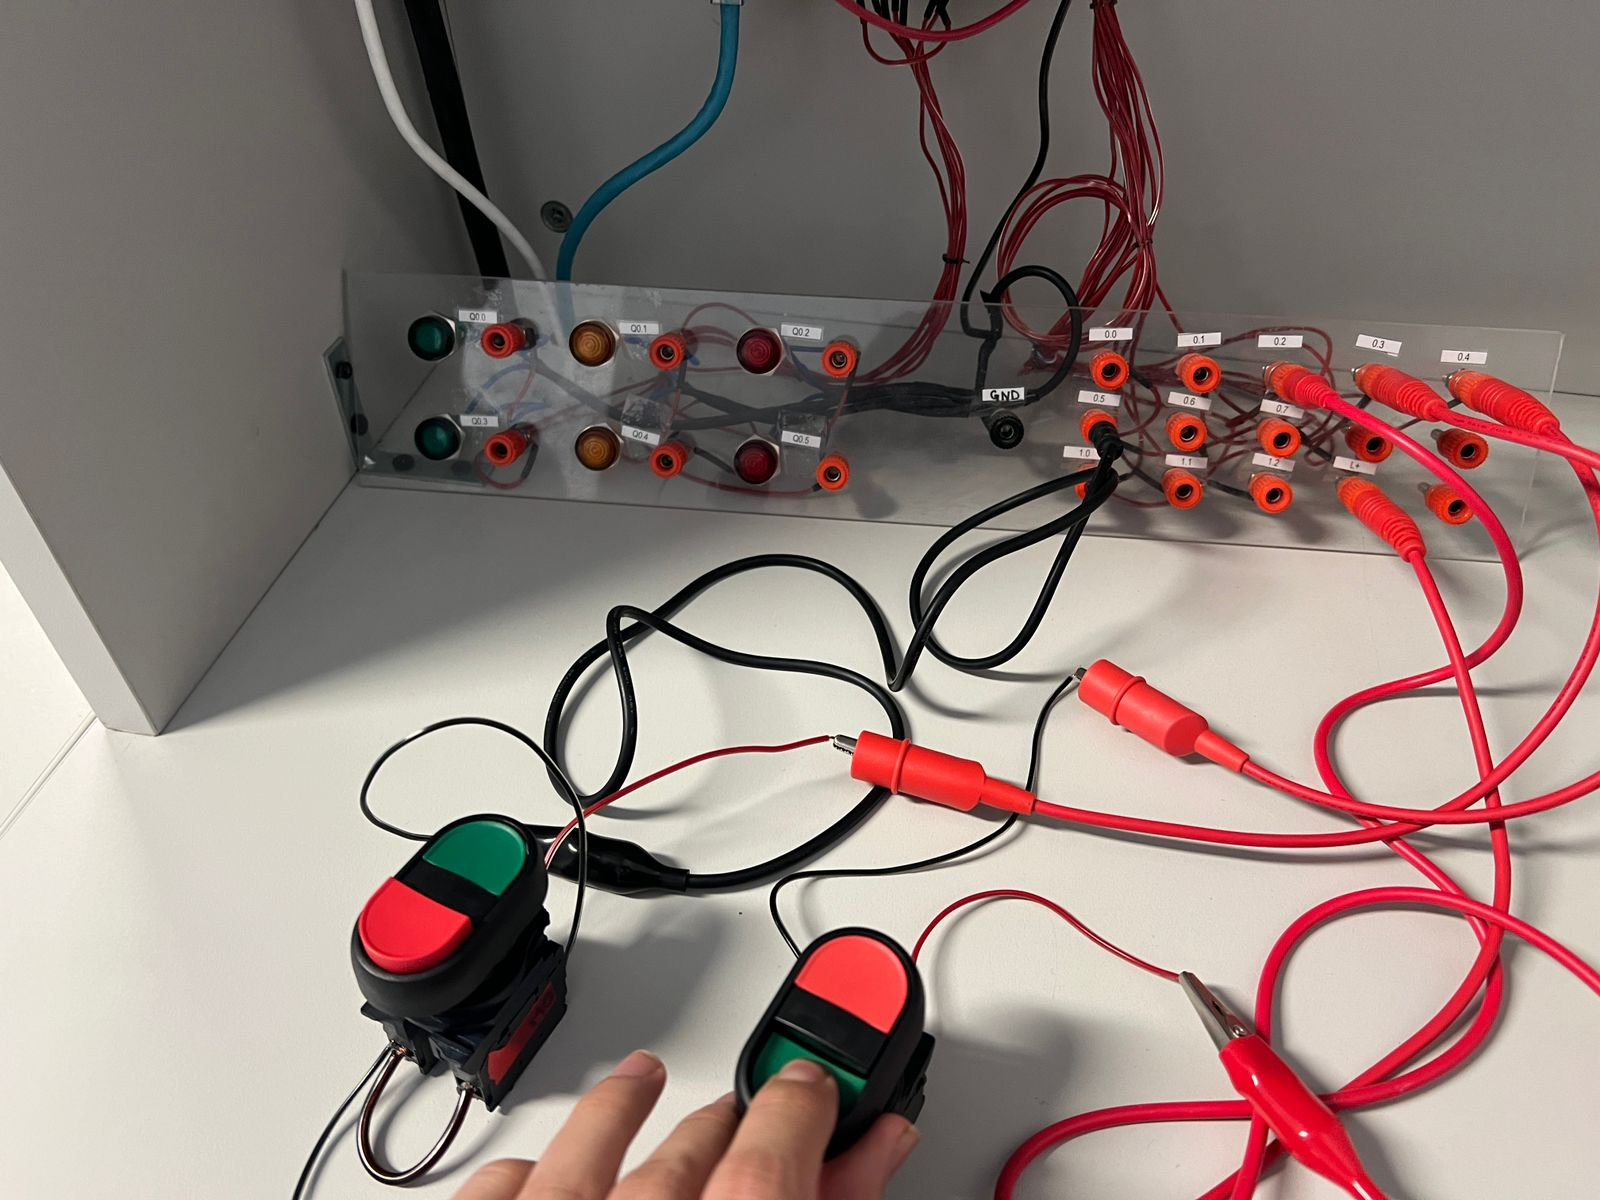
\includegraphics[width=\textwidth]{screenshots/imagen_2.jpg}
      \caption{Reset}
      \label{fig:apagado}
    \end{minipage}
  \end{figure}
\end{enumerate}






\newpage

%----- CONCLUSIONES ----
\chapter{Conclusiones}
En esta práctica, se implementó y simuló un circuito de interbloqueo utilizando el software adecuado. A través de la creación de variables de entrada y salida, así como la configuración correcta de los componentes del circuito, se pudo verificar el funcionamiento del interbloqueo.

El interbloqueo eléctrico demostró ser una técnica efectiva para asegurar que solo una salida esté activa a la vez, previniendo así posibles daños en el sistema y mejorando la seguridad operativa. La simulación permitió observar cómo el circuito de interbloqueo impide la activación simultánea de dos salidas, lo cual es crucial en aplicaciones industriales donde la coordinación y la seguridad son primordiales.

\newpage


\end{document}